En esta sección se presentarán diversos artículos de investigación o tesis las cuales abordarán diversas técnicas y enfoques que se emplearon para afrontar problemas similares al de esta tesis. Asimismo, a continuación se presenta un cuadro resumen (véase Anexo \ref{A:table}) de lo que se presenta en esta sección.


\subsection{A Chatbot for Information Security  \citep*{pr_A_Chatbot_for_Information_Security}}

\citeauthor{pr_A_Chatbot_for_Information_Security} realizó un artículo de investigación el cual fue publicado en la revista «IJCSNS International Journal of Computer Science and Network Security» en el año 2020. 
Este fue titulado \citetitle{pr_A_Chatbot_for_Information_Security} la cual traducida al español significa «Un chatbot para la seguridad de la información».

\subsubsection{Planteamiento del Problema y objetivo }
El artículo aborda el asesoramiento sobre seguridad de la información y se centra en la creación de una interfaz backend qué interactua con una base de datos de conocimientos( Preguntas y respuestas a consultas previas ). El problema planteado se relaciona con la necesidad de comprender cómo los chatbots pueden ayudar a la atención de clientes y su uso como asistente digital para mejorar la satisfacción del cliente y, en última instancia, impulsar el rendimiento de las empresas.

\subsubsection{Fundamento Teórico usado por el Autor}
El autor planteó emplear una combinación entre la función de PLN (Procesamiento del Lenguaje Natural) basado en el texto y los chatbots basados en la nube para la creación de su chatbot propuesto.

\subsubsection{Metodología empleada por los autores}
La metodología empleada por el autor, para la creación de su chatbot consiste en 4 pasos: 

\begin{enumerate}
    \item Captura los datos imputados por parte del cliente en el área de Frontend de la página web.
    \item Realiza una busqueda de en la base de datos a partir de las palabras clave extraidas de los datos imputados.
    \item Retorna las respuestas que mejor se asemejan a la pregunta y palabras claves asociadas a la misma.
    \item Envía al cliente la respuesta que mejor se asemeje a un caso similar a la pregunta o cunsulta ingresada.
\end{enumerate}

\begin{figure}[h]
	\begin{center}
		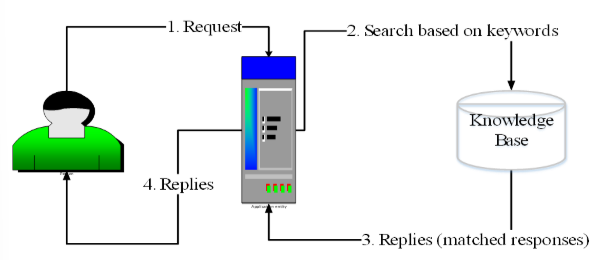
\includegraphics[width=1\textwidth]{2/figures/1_1.png}
		\caption{Arquitectura propuesta para el chatbot (\cite{pr_A_Chatbot_for_Information_Security})}
	\end{center}
\end{figure}

\begin{figure}[h]
	\begin{center}
		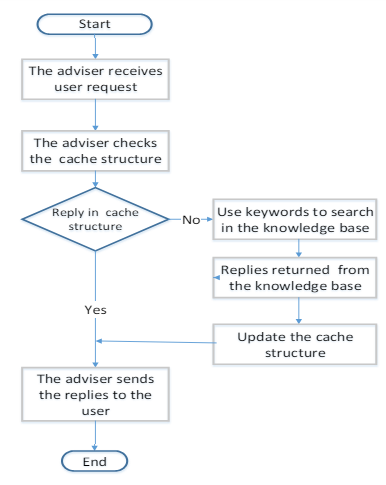
\includegraphics[width=0.50\textwidth]{2/figures/1_2.png}
		\caption{Acciones seguidas por el chatbot propuesto (\cite{pr_A_Chatbot_for_Information_Security})}
	\end{center}
\end{figure}

\subsubsection{Resultados obtenidos}
En el paper, se desarrolla un chatbot que extrae las palabras claves a lo largo de su conversación con los usuarios, para luego utilizar estas palabras claves en su base de datos de conocimientos (en un archivo JSON) y le envía las respuestas con más similitudes en su base de datos. 
Se resalta la ventajas adquiridas por la implementación del chatbot como la respuesta acertada para el usuario en un corto. Asimismo se destaca su intensión de implementar el chatbot en otras plataformas, considerando a Telegram como una de sus alternativas de aplicación futura.

%%%%%%%%%%%%%%%%%%%%%%%%%%%%%%%%%%%%%%%%%%%%%%%%%%%%%%%%%%%%%%%%%%%%%%%%%%%%%%%%%%%%%%%%%%%%%%%%%%%%%%%%%%%%%%%%%%%%%%%%%%%%
\subsection{Implementation of a chatbot in Azure
integrated with Teams \& Dynamics  \citep*{ts_ICAITD}}

\citeauthor{ts_ICAITD} realizó un trabajo de fin de grado el cual fue publicado en base de datos de su universidad «Universidad de Cantabria» en el año 2021. 
Este fue titulado \citetitle{ts_ICAITD} la cual traducida al español significa «Implementación de un chatbot en Azure
integrado con Teams y Dynamics».

\subsubsection{Planteamiento del Problema y objetivo }
La investigación aborda la ayuda al usuario con sus tareas cotidiantes a través del CRM ( Customer Relationship Management ) de CIC ( Consulting Informático ). 
Los gerentes como responsables del CIC, los cuales a su vez realizan diversas tareas relacionadas con el CRM, persiben un problema constante, el cual radica en el conocimiento requerido para conocer las distintas interfaces de la plataforma de Dynamics. Razón por la cual se propone un chatbot para agilizar el uso de las distintas interfaces en un menor tiempo.

\subsubsection{Fundamento Teórico usado por el Autor}

El autor plantea emplear Visual Studio Enterprise 2019 y el entorno web proporcionado por Microsoft, el lenguaje LUIS (Language Understanding), la cual es un servicio de inteligencia conversación. Asimismo, se indica utilizar el portal de Azure para el almacenamiento de la información.

\begin{figure}[h]
	\begin{center}
		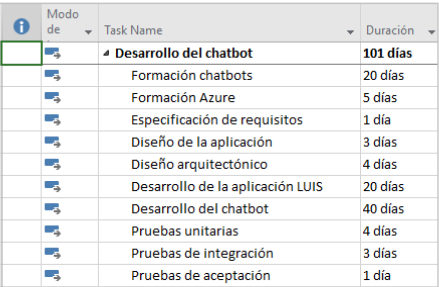
\includegraphics[width=0.6\textwidth]{2/figures/2_1.png}
		\caption{Diagrama de Gantt \- Parte 1 (\cite{ts_ICAITD})}
	\end{center}
\end{figure}

\begin{figure}[h]
	\begin{center}
		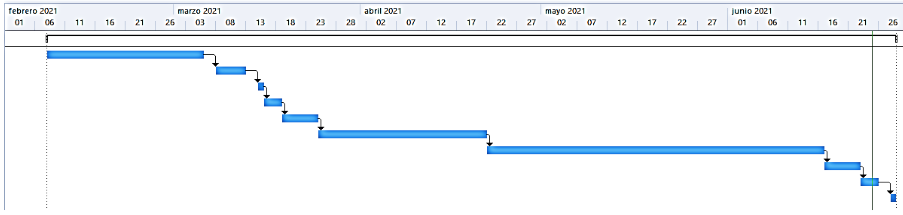
\includegraphics[width=1\textwidth]{2/figures/2_2.png}
		\caption{Diagrama de Gantt \- Parte 2 (\cite{ts_ICAITD})}
	\end{center}
\end{figure}


\subsubsection{Metodología empleada por los autores}
La metodología empleada por el autor, para la creación de su chatbot consiste en los siguientes pasos: 

\begin{enumerate}
    \item Captura los datos imputados por parte del cliente, la petición, en el área de Frontend de la página web.
    \item Autentica al usuario y autoriza la petición, gracias a Azure, retornando su llave (token).
    \item Realiza una consulta procesada por LUIS.
    \item Retorna los resultados que mejor se asemejan, procesado por LUIS.
    \item Luego de obtener los resultados se almacena los logs correspondientes  y "feedback" necesario para el monitoreo y los reportes.
    \item Envía al cliente o usuario la respuesta.
\end{enumerate}

\begin{figure}[h]
	\begin{center}
		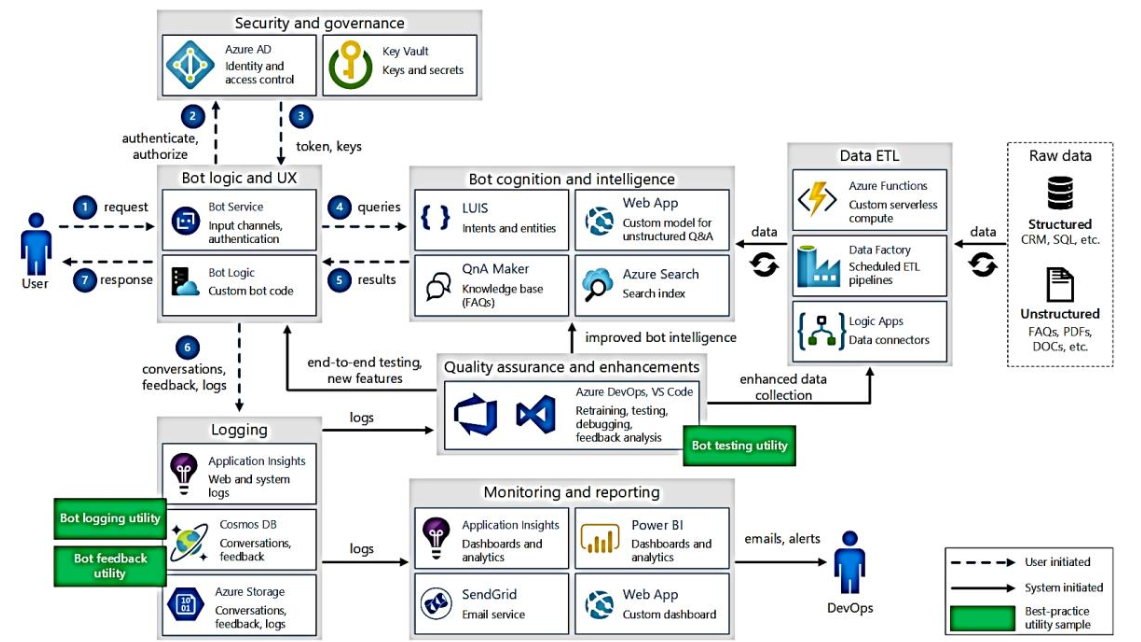
\includegraphics[width=1\textwidth]{2/figures/2_3.png}
		\caption{Arquitectura del bot de Azure (\cite{ts_ICAITD})}
	\end{center}
\end{figure}

\subsubsection{Resultados obtenidos}
A lo largo del tabajo se desarrolla un chatbot integrado con Teams y Dynamics para hace más sencillo el uso del CRM por parte de los empleados de CIC. El chatbot posee varias funcionalidades como, consultar registros del CRM, obtener las oportunidades proximas a caducar, visualizar las últimas oportunidades creadas y consultar a su vez los estados de la misma. \\
Se resalta la facilidad del trabajo por parte de todos los usuario del CRM de CIC, el nivel de eficiencia mayor obtenida por su implementación, al ser más rápida y eficiente, y el potencial que puede tener con los proximos usuarios y las funcionalidades que se le puedan añadir debido a cambios en el CRM.

%%%%%%%%%%%%%%%%%%%%%%%%%%%%%%%%%%%%%%%%%%%%%%%%%%%%%%%%%%%%%%%%%%%%%%%%%%%%%%%%%%%%%%%%%%%%%%%%%%%%%%%%%%%%%%%%%%%%%%%%%%%%

\subsection{Chatbot con Dialogflow y Redes Neuronales Recurrentes para la mejora del proceso de comercialización de productos agrícolas para la gerencia regional de agricultura \citep*{ts_CDRNRMPC}}

\citeauthor{ts_CDRNRMPC} realizó un trabajo de fin de grado el cual fue publicado en base de datos de su universidad «Universidad de Cantabria» en el año 2021. 
Este fue titulado \citetitle{ts_CDRNRMPC}.

\subsubsection{Planteamiento del Problema y objetivo }

La investigación aborda la necesidad de mejorar el proceso de comercialización de los productos agrícolas a la hora de venderlos mediante el uso de sistemas conversacionales e Inteligencia Artificial. Por ello, su objetivo se enfoca en el despliegue de un chatbot impulsado con el servicio Dialogflow y redes neuronales para solventar la necesidad encontrada.

\subsubsection{Fundamento Teórico usado por el Autor}

El autor plantea hacer uso de Dialogflow, platafroma para desarrollo de chatbots y agentes virtuales, y redes neuronales recurrentes, para el análisis de datos de series temporales. Para la captura de la información recurrió a entrevistas, encuestas y capacitaciones, para poder determinar las funcionalidades que podrían añadirse al chatbot a desarrollar.

\subsubsection{Metodología empleada por los autores}
La metodología empleada por el autor, para la creación de su chatbot consiste en los siguientes pasos: 

\begin{enumerate}
    \item Captura los datos imputados por parte del cliente.
    \item Envía el query a Dialogflow para su procesamiento.
    \item Se procesa la información mediante una API externa y el código implementado, así como la base de datos.
    \item Retorna los resultados procesados y se agrega información extra requerida.
    \item Envía al cliente o usuario la respuesta.
\end{enumerate}

\begin{figure}[h]
	\begin{center}
		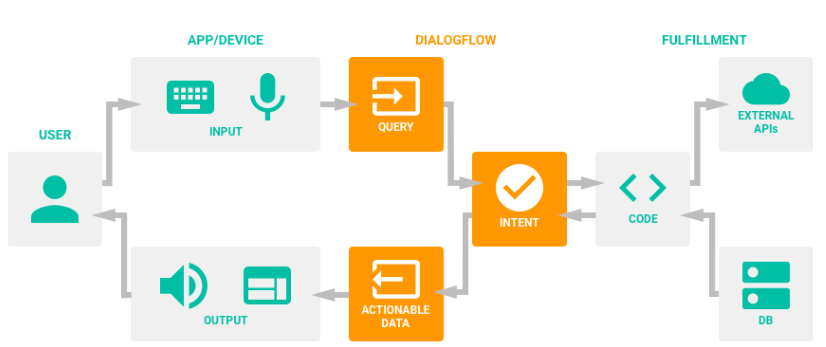
\includegraphics[width=1\textwidth]{2/figures/3_1.png}
		\caption{Diagrama de flujo de Dialogflow(\cite{ts_CDRNRMPC})}
	\end{center}
\end{figure}

\subsubsection{Resultados obtenidos}

A lo largo del trabajo se comprobó el problema durante la ejecución del proceso de agricultores, las cuales eran inconsistencia de datos, largos tiempos de espera por parte de la gerencia agraria y respuestas erróneas por parte de la misma. Estos problemas pudieron ser cubiertos por la implementación del chatbot propuesto impulsado por NLP y Dialogflow, el cual posteriormente mostró indicadores de beneficio, como encontrar un 90\% de agricultores que mejoraron su proceso de comercialización agrícola, a la par que 50\% de los agricultores mejoró su rendimiento en un 95\%.
Se resalta también la confiabilidad, satisfacción, diseño y usabilidad que posee el chatbot, mostrando a su vez una percepción positiva entre los usuarios.

%%%%%%%%%%%%%%%%%%%%%%%%%%%%%%%%%%%%%%%%%%%%%%%%%%%%%%%%%%%%%%%%%%%%%%%%%%%%%%%%%%%%%%%%%%%%%%%%%%%%%%%%%%%%%%%%%%%%%%%%%%%%

\subsection{Design and Development of AI-Powered Healthcare 
WhatsApp Chatbot \citep*{pr_DDAIHWC}}

\citeauthor{pr_DDAIHWC} realizó un artículo publicado en base de datos de la IEEE «Institute of Electrical and Electronics Engineers» en el año 2023.
Este fue titulado \citetitle{pr_DDAIHWC} la cual traducida al español significa «Diseño y desarrollo de chatbot de WhatsApp para el sector sanitario impulsado por IA». 

\subsubsection{Planteamiento del Problema y objetivo }

La investigación aborda la necesidad de crear un chatbot artificial para hacer un chat en vivo tanto los usuarios como los pacientes de forma conjunta con respecto a las citas médicas con los médicos interesados, de forma que puede ser un proyecto escalable B2C e incluso B2B. Por ello, su objetivo se enfoca en la creación de un chatbot impulsado  PLN (Procesamiento de Lenguaje Natural) para solventar la necesidad encontrada.

\subsubsection{Fundamento Teórico usado por el Autor}

Los autores plantean utilizar el PLN como herramienta principal en la creación del chatbot, la cual a su vez utilizará una RNN (Red Neuronal Recurrente) para el mapeo de las palabras claves y el contexto de la pregunta, ajustando según se requiera los parámetros de aprendizaje. Asimismo, utiliza el BPTT (Backpropagation Through Time), la cual toma en consideración la secuencia ordenada del input y output.

\subsubsection{Metodología empleada por los autores}
La metodología empleada por el autor, para la creación de su chatbot consiste en los siguientes pasos: 

\begin{enumerate}
    \item El usuario envía un mensage en WhatsApp.
    \item En caso de estar registrado manda la consulta a la base de datos para procesarse, caso contrario envía un mensaje de registro al usuario.
    \item De la base de datos se envía a la página del chatbot para ser procesado.
    \item En el procesamiento es mapeado y se le otorga contexto  mediante RNN, pasa por BPTT para terminar el procesamiento del mensaje y enviar el resultado procesado.
    \item Retorna el resultado procesado y se envía al cliente o usuario la respuesta.
\end{enumerate}

\begin{figure}[h]
	\begin{center}
		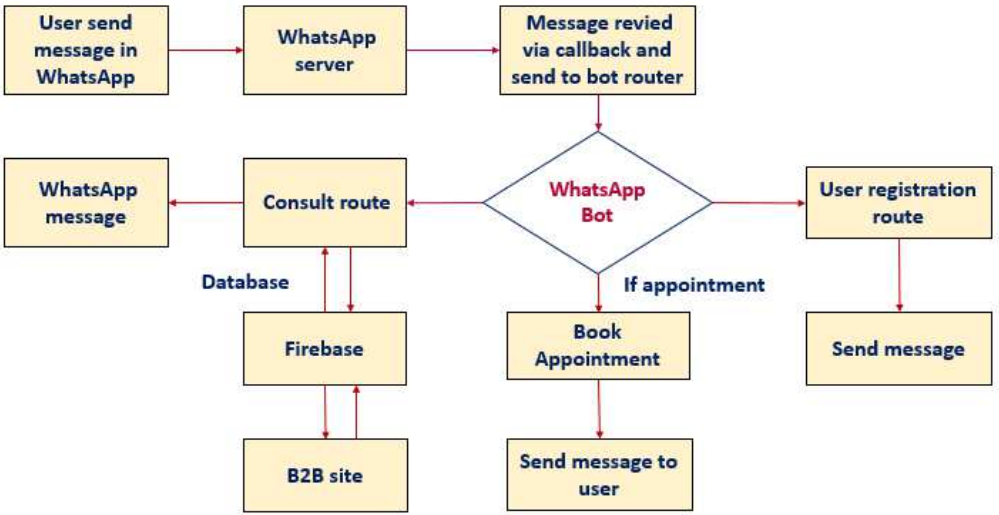
\includegraphics[width=1\textwidth]{2/figures/4_1.png}
		\caption{Diagrama de flujo del chatbot(\cite{pr_DDAIHWC})}
	\end{center}
\end{figure}

\subsubsection{Resultados obtenidos}

Como resultado en el trabajo se destacan la disponibilidad de los servicios de cuidado ( alertas médicas, soporte de clientes y vacunas ) de salud en todo momento. Asimismo, se resalta la ayuda que proporciona el chatbot en el seguimiento del cuidado de la salud de los clientes y el potencial que posee para transformar la industria de atención médica al hacer más eficiente y rápida el acceso a los servicios médicos, la cual se destaca en la atención en tiempo real, métodos de pago, atención e informe de la información del paciente y la asistencia a los mismos con recordatorios.

%%%%%%%%%%%%%%%%%%%%%%%%%%%%%%%%%%%%%%%%%%%%%%%%%%%%%%%%%%%%%%%%%%%%%%%%%%%%%%%%%%%%%%%%%%%%%%%%%%%%%%%%%%%%%%%%%%%%%%%%%%%%


\subsection{Artificial Intelligence Powered Chatbot for Mental Healthcare based on Sentiment Analysis \citep*{pr_AIPCMHBSA}}

\citeauthor{pr_AIPCMHBSA} realizó un artículo publicado en base de datos de la IEEE «Institute of Electrical and Electronics Engineers» en el año 2022.
Este fue titulado \citetitle{pr_AIPCMHBSA} la cual traducida al español significa «Chatbot impulsado por inteligencia artificial para el cuidado de la salud mental basado en el análisis de sentimientos». 

\subsubsection{Planteamiento del Problema y objetivo }

El artículo aborda principalmente el problema del cuidado de la salud mental y la dificultad en la detección y el tratamiento del mismo, razón por la cual se ha tornado relevante la creación de aplicaciones para el cuidado mental de la persona, la cual se incrementó en un 31.9\% el 2022 comparado al 2021. En búsqueda de que las personas se abran sin miedo a ser juzgados por sus problemas, se plantea un chatbot el cual pueda entender las emociones de los usuarios a partir de un análisis de los sentimientos, para proveer respuestas personalizadas a los usuarios.

\subsubsection{Fundamento Teórico usado por el Autor}

Los autores para el desarrollo y procesamiento del chatbot plantean utilizar el Bidirectional LSTM ( Long Short Term Memory Networks), la cual permite un análisis de los datos y predecir de forma lineal y en reversa, mejorando el rendimiento del mismo en el análisis de los sentimientos.
Asimismo para el análisis de sentimientos se realiza una ANN (Artificial Neuronal Network) la cual se utiliza para la contextualización de la conversación y la clasificación de los mensajes mediante distintas categorías.

\begin{figure}[h]
	\begin{center}
		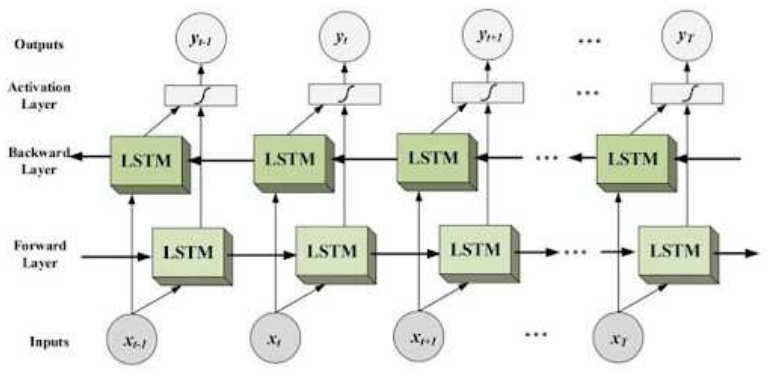
\includegraphics[width=1\textwidth]{2/figures/5_1.png}
		\caption{Bidirectional LSTM (\cite{pr_AIPCMHBSA})}
	\end{center}
\end{figure}

\subsubsection{Metodología empleada por los autores}
La metodología empleada por los autores, para la creación de su chatbot consiste en los siguientes pasos: 

\begin{enumerate}
    \item El usuario envía un mensage en WhatsApp.
    \item Se inicia el procesamiento de la destaca
    \item Se le asigna un tag y se analiza la intensión del mensaje 
    \item Categoriza a la par que se provee información por parte del modelo ANN y se contextualiza el tag y prevee el nivel del sentimiento mediante el modelo bidireccional LSTM.
    \item Una vez realizado el análisis se compone la respuesta del chatbot.
    \item Se envía el mensaje al usuario.
\end{enumerate}

\begin{figure}[h]
	\begin{center}
		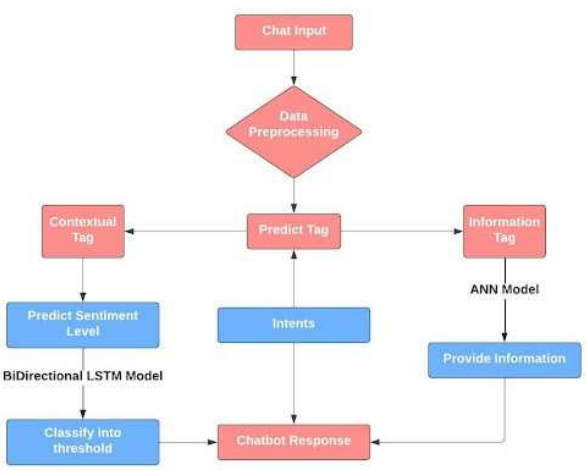
\includegraphics[width=0.8\textwidth]{2/figures/5_2.png}
		\caption{Diagrama de flujo del chatbot(\cite{pr_AIPCMHBSA})}
	\end{center}
\end{figure}

\subsubsection{Resultados obtenidos}
Como resultado de la implementación y el análisis de los mensajes de 140 datasets de tweets se obtuvo un accuracy de 80.88\%, logrando detectar los sentimientos negativos y positivos a la par de las dobles negaciones en algunos mensajes. El chatbot creado provee un pérdida mínima de 0.0185 lo cual indica que puede contextualizar con exito los tags y clasificaciones asignadas a distintos mensajes. Asimismo, el chatbot puede identificar correctamente un contexto de ansiedad por parte del usuario al cual el chatbot ofrece ayuda para conocer más de sus sentimientos.
Se resalta que la implementación de un chatbot para el cuidado mental de las personas, impulsado por IA \& ML es de mucha utilidad para proveer respuestas apropiadas, según el contexto sentimental que tiene el chat. Además, se resalta la intención de desarrollar mejor el chatbot con elementos más complejos, como algoritmos.

%%%%%%%%%%%%%%%%%%%%%%%%%%%%%%%%%%%%%%%%%%%%%%%%%%%%%%%%%%%%%%%%%%%%%%%%%%%%%%%%%%%%%%%%%%%%%%%%%%%%%%%%%%%%%%%%%%%%%%%%%%%%

%%%%%%%%%%%%%%%%%%%%%%%%%%%%%%%%%%%%%%%%%%%%%%%%%%%%%%%%%%%%%%%%%%%%%%%%%%%%%%%%%%%%%%%%%%%%%%%%%%%%%%%%%%%%%%%%%%%%%%%%%%%%

%%%%%%%%%%%%%%%%%%%%%%%%%%%%%%%%%%%%%%%%%%%%%%%%%%%%%%%%%%%%%%%%%%%%%%%%%%%%%%%%%%%%%%%%%%%%%%%%%%%%%%%%%%%%%%%%%%%%%%%%%%%%

%%%%%%%%%%%%%%%%%%%%%%%%%%%%%%%%%%%%%%%%%%%%%%%%%%%%%%%%%%%%%%%%%%%%%%%%%%%%%%%%%%%%%%%%%%%%%%%%%%%%%%%%%%%%%%%%%%%%%%%%%%%%

%%%%%%%%%%%%%%%%%%%%%%%%%%%%%%%%%%%%%%%%%%%%%%%%%%%%%%%%%%%%%%%%%%%%%%%%%%%%%%%%%%%%%%%%%%%%%%%%%%%%%%%%%%%%%%%%%%%%%%%%%%%%

% %%%Ecuacion
% \begin{equation}  
% \label{eq:RMSE}
% RMSE = \sqrt{\frac{\sum_{i=1}^{N}{\Big(O_i -T_i\Big)^2}}{N}}
% \end{equation}